\negspace
In the current section we present our framework for scalable and NUMA-aware producer-consumer data exchange. 
Our system follows the principle of separating mechanism and policy.
We therefore consider two independent logical entities: 
\snegspace
\begin{enum*}
	\item \emph{A single consumer pool (SCPool)} mechanism manages the tasks arriving to a given consumer and allows tasks stealing by other consumers.
	\item A management policy operates SCPools: it routes producer requests to the appropriate consumers and initiates stealing between the pools. This way, the policy controls the system's behavior according to considerations of load-distribution, throughput, fairness, locality, etc.
	We are especially interested in a management policy suitable for NUMA architectures (see Figure~\ref{fig:system-fig}), where each CPU has its own memory, and memories of other CPUs are accessed over an interconnect. As a high rate of remote memory accesses can decrease the performance, it is desirable for the SCPool of a consumer to reside close to its own CPU. 
\end{enum*} 

\negspace
\paragraph{SCPool abstraction.}
\begin{algo}[!ht]
\caption{API for a Single Consumer Pool with stealing support.} 
\label{alg:scpool-api}
\begin{distribalgo}[1]
\scriptsize

\INDENT {\bf SCPool API:}
	\STATE produce(Task) \elcomment {Insert the task to the pool, returns false if no space left in the pool.}
	\STATE produceForce(Task) \elcomment {Inserts the task to the pool, expanding the pool if necessary. }
	\STATE consume() \elcomment {Retrieves a task from the pool, returns $\bot$ if no tasks in the pool are detected.}
	%\STATE getStealingScore() \elcomment {Returns a score corresponding to the amount of tasks to steal.}
	\STATE steal(SCPool from) \elcomment{Tries to steal a number of tasks from the given pool and move them to the current pool. Returns one of the stolen tasks or $\bot$. }%We guarantee that if there are tasks in the \emph{from} pool at the beginning of steal invocation, then either steal function returns a task, or there is another thread that returns a task during the steal execution.}
\ENDINDENT

\end{distribalgo}
\end{algo}

The SCPool API provides the abstraction of a single-consumer task pool with stealing support, see Algorithm~\ref{alg:scpool-api}.
A producer can invokes two operations: {\bf produce()}, which attempts to insert a task to the given pool and fails if the pool is full, and {\bf produceForce()}, which always succeeds by expanding the pool on demand.
There are also two ways to retrieve a task from the pool: the owner of the pool (only) can call the {\bf consume()} function; while any other thread can invoke {\bf steal()}, which tries to transfer a number of tasks between two pools and return one of the stolen tasks. 
% The pool must guarantee the following \emph{stealing property}, which is necessary for system liveness:
% \begin{property}
% \label{steal-progress-property}
% If an SCPool is not empty at the beginning of a steal operation, then either the steal operation retrieves a task, or another thread started an operation $op$ during the steal execution, such that $op$ is guaranteed to retrieve a task.
% \end{property}

A straightforward way to implement the above API is using dynamic-size multi-producer multi-consumer FIFO queue (e.g., Michael-Scott queue~\cite{Michael:1996:SFP:248052.248106}).
In this case, {\bf produce()} enqueues a new task, while {\bf consume()} and {\bf steal()} dequeue a task. In the next section we present SALSA, a much more efficient SCPool.

%\begin{wrapfigure}{l}{0.5\textwidth}
%  \vspace{-20pt}
%  \begin{center}
%    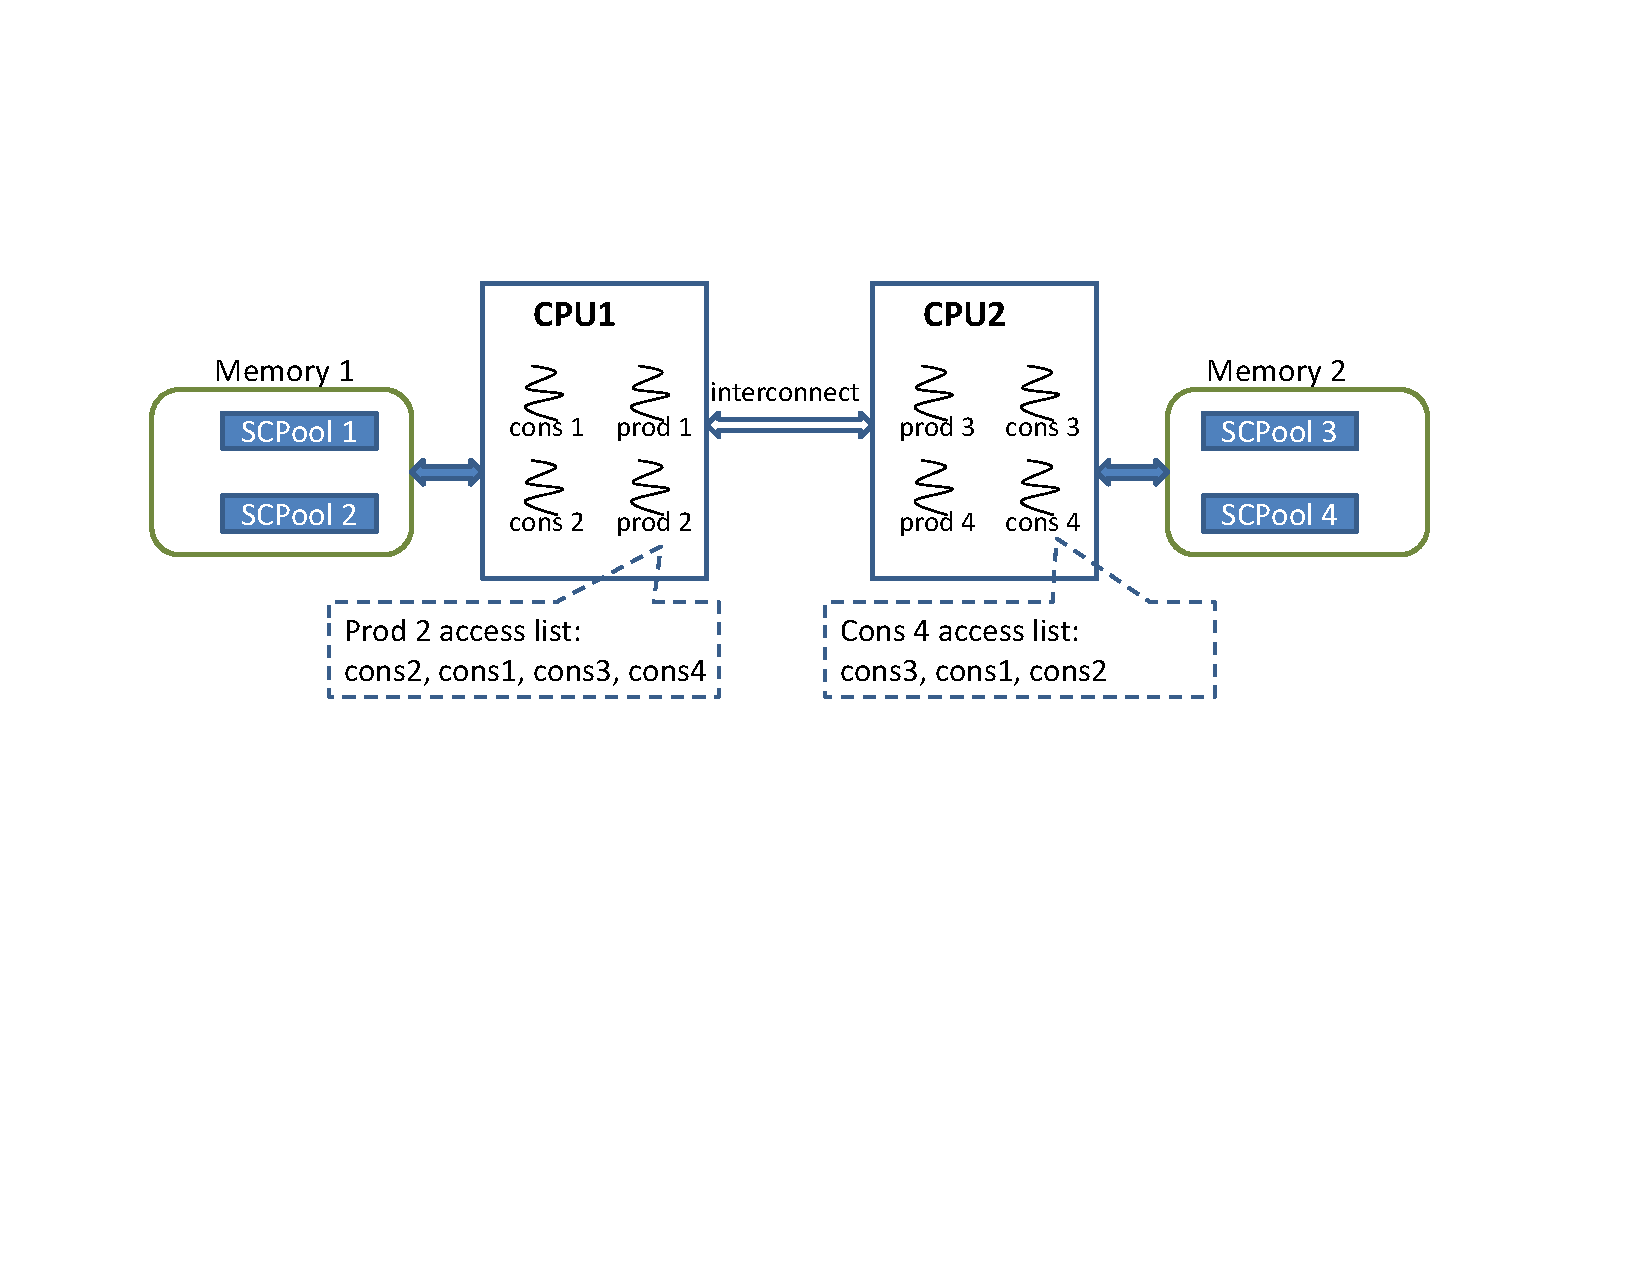
\includegraphics[width=0.48\textwidth]{figures/system-fig}
%  \end{center}
%  \vspace{-20pt}
%  \caption{\footnotesize{Producer-consumer system overview. In the given example, the system is composed of two processors connected to two memory banks (NUMA architecture). There are two producers and two consumers running on each processor, and the data of each consumer is allocated at the closest available physical memory. A producer $p_i$ has an access list of consumers for task insertion. A consumer $c_i$ has an access list of consumers for task stealing.}}
%  \vspace{-10pt}
%  \label{fig:system-fig}
%\end{wrapfigure}

\begin{figure}[htb]
	\centering
	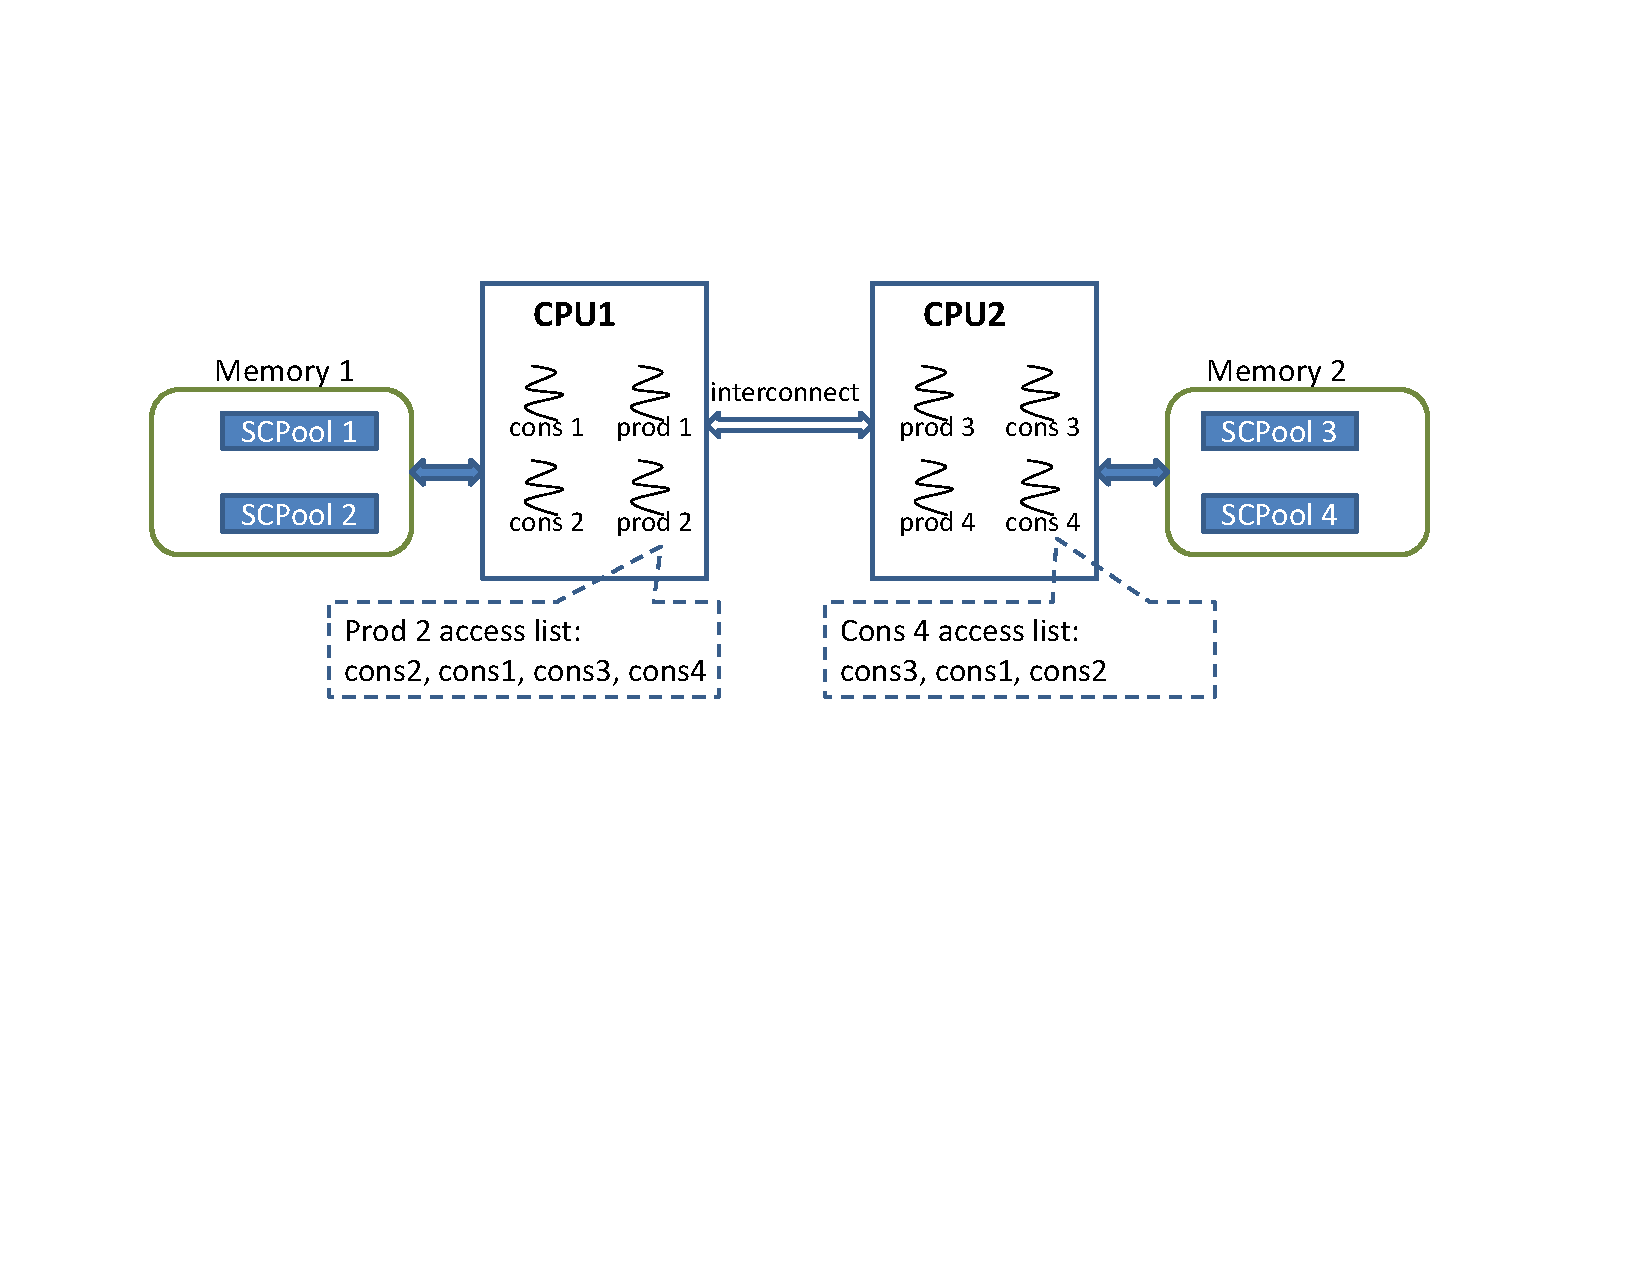
\includegraphics[width=0.6\textwidth]{figures/system-fig}
	\caption{\footnotesize{Producer-consumer framework overview. In this example, there are two processors connected to two memory banks (NUMA architecture). Two producers and two consumers running on each processor, and the data of each consumer is allocated at the closest physical memory. A producer (consumer) has a sorted access list of consumers for task insertion (respectively stealing). }}
	\label{fig:system-fig}
\end{figure}

\negspace
\paragraph {Management policy.}
A management policy defines the way in which: 1) a producer chooses an SCPool for task insertion; and 2) a consumer decides when to retrieve a task from its own pool or steal from other pools. 
Note that the policy is independent of the underlying SCPool implementation. We believe that the policy is a subject for engineering optimizations, based on specific workloads and demands.

In the current work, we present a NUMA-aware policy. If the individual SCPools themselves are lock-free, then our policy preserves lock-freedom at the system level. Our policy is as follows:
\snegspace
\begin{item*}
	\item {\bf Access lists.} Each process in the system (producer or consumer) is provided with an \emph{access list}, an ordered list of consumers, sorted according to their distance from that process (see Figure~\ref{fig:system-fig}). Intuitively, our intention is to have a producer mostly interact with the closest consumer, while stealing mainly happens inside the same processor node. 
	\item {\bf Producer's policy.} A producer first calls the {\bf produce()} of the first SCPool in its access list. Note that this operation might fail if the pool is full, (which can be seen as evidence of that the corresponding consumer is overloaded).  In this case, the producer tries to insert the task into other pools, in the order defined by its access list. If all insertions fail, the producer invokes {\bf produceForce()} on the closest SCPool, which always succeeds (expanding the pool if needed). 
	\item {\bf Consumer's policy.} A consumer takes tasks from its own SCPool. If its SCPool is empty, the consumer tries to steal tasks from other pools in the order defined by its access list. The issue of when (after how many stealing attemps) a consumer gives up and returns $\bot$ is subtle, and we discuss it in Section~\ref{sec:correctness}. Stealing serves two purposes: first, it is important for distributing the load among all available consumers. Second, it ensures that tasks are not lost in case they are inserted into  the SCPool of a crashed (or  very slow) consumer.
\end{item*}
